\section{Agent Society Overview}
\label{sec:society}

In this section we present the structure of the agent society and the argumentation framework used in interaction between agents. First our argumentation framework consists of a number of intelligent agents capable of exchanging arguments using the AIF\cite{aif}. These agents can understand human language and are able to extract arguments from text in English. In addition to the AIF at least one topic ontology is needed in the framework to provide the ground knowledge accepted by all agents in the system. Note that the society is not constrained to use a specific ontology as a whole, but rather each agent needs at least one ontology. This allows agents to play different roles in the society analogous to the roles humans play in our society. For example an agent may have several ontologies describing legal concepts, while other agent may only know about animals. In this approach ontologies shared by all agents represent a limited form common sense knowledge. As we will see in section[\ref{sec:application}] the framework can be augmented with additional capabilities to retrieve data from external sources and insert it into AIF. 

Humans can also take part in a debate using English language. A human can debate on a given topic with one or more agents. As shown in section[\ref{sec:application}] each agent has it's own behavior and different agents may accept different arguments as valid based on their knowledge and various behavior parameters. In a debate each agent maintains an own view of the argumentation and will try at best to attack and defend arguments based on it's own position in the debate. If an agent can't determine the acceptability of an argument he may ask other agents. This is a two step process involving a query to the Facilitator  which returns a list of agents discussing on a given topic. In the next step a query is sent to all agents that might know about this argument. If an agent knows the accessibility value of the property of the argument than an additional query can be made for an argumentation schema. This process may continue in a manner similar to a backward-chaining proof. Note that this process involves agents that share at least one ontology, other than AIF. Because of this agents may form interest groups in the society and interactions only occur within these groups.

\section{Agent Architecture}
\label{sec:application}

In this section we present the architecture of the agent. Each agent can understand natural language and interact with humans and other agents. The NLP module is used to create a schema of argumentation from the text. This schema is used by the reasoning module to determine the argumentation plan and the admissibility of arguments using Dung acceptability\cite{dung}. Each agent has also an associated behavior that is essentially a set of parameters that control the algorithms used in the reasoning module. Finally each agent has a communication module used to interact with other agents as described in section[\ref{sec:society}].
\par
Although the use of an ontology has many advantages over other sources of information, such a database or a knowledge base the AIF does not enforce the structure of the domain knowledge used by agents. Because of this any agent can be augmented with capabilities for extracting knowledge. This can be used to support the admissibility of arguments.
In this section we present the architecture of the agent. At the top level we have build an autonomous intelligent agent that has it's own behavior module and reasoning capabilities. Moreover each agent can understand natural language and interact with humans and other agents.

\begin{figure}[t]
\centering
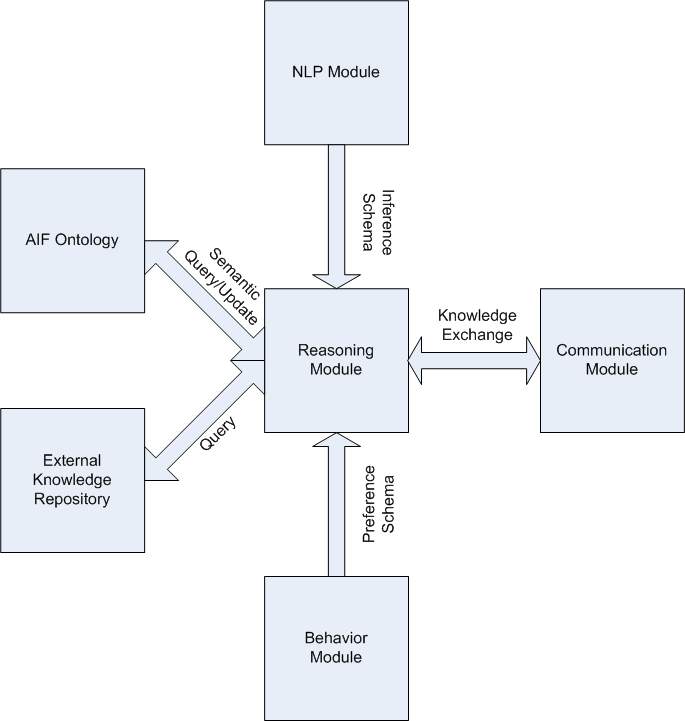
\includegraphics[scale=0.47]{TopLevelAgentStructure}
\caption{Top Level Agent Architecture}
\label{fig:arch}
\end{figure}

\subsection{NLP Module Description}

The NLP (Natural Language Processing) module is an important component of the overall agent architecture. Its role gains significant attention in the scenario where a human counterpart is engaged in a debate with one or several agents.
In such a setting, the human counterpart will communicate with the agent system using the English language. An individual engaged in a debate will enter text that defines his current standpoint in the entire argumentation process.
The purpose of the NLP module then becomes that of parsing this text and of producing an internal representation of the current argument intended by the user. The output of the module will consist in an inference scheme which will be used by the main reasoning module of each agent to update its current beliefs and behavior (the way in which it will possibly try to being a counter-argument). The next section will provide a detailed description of this module as well as the results obtained.

\subsection{AIF Ontology}

The Argument Interchangeable Format(AIF)\cite{aif} is an ontology designed for exchanging arguments between different software applications. In particular it can be used in a multi agent system to provide support for argumentation between agents. As it is shown in \cite{aif} the representation of arguments using AML\cite{araucaria}\cite{reed} schemas can be directly mapped into this ontology.
\par
The core of AIF consists of a set of definitions for high level concepts related to argumentation that are represented in the ontology.These concepts are divided into three main groups:
\begin{itemize}
\item \textit{Arguments and Argument Networks}: the core ontology for argument entities and relations between argument entities.
\item \textit{Communication}: the core ontology for items which relate to the interchange of arguments between two or more participants in an environment, including locutions and protocols.
\item \textit{Context}: the core ontology for items associated with environments in which argumentation may take place. These include participants in argument exchanges (agents), theories contained in the environment that are used for argumentation, and other aspects which may affect the meaning of arguments/communication of arguments.
\end{itemize}
The following figure from \textit{http://www.x-opennet.org/aif/Inputs/aif2005\_}
\newline
 \textit{david\_hitchcock\_1.pdf} shows the relations between main components of AIF ontology:

\begin{figure}[tbh]
\centering
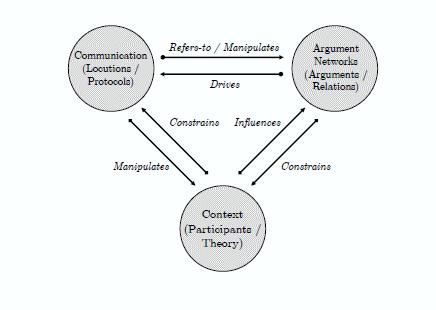
\includegraphics{aifs1.jpg}
\caption{Relations between main components in AIF}
\label{fig:aif1}
\end{figure}

The main entities used from AIF are summarized below. For a detailed discussion of these see\cite{aif}:
\begin{table}[tbh]
\centering
\begin{tabular}{|p{2.3cm}|p{2.3cm}|p{2.3cm}|p{2.3cm}|p{2.3cm}|}
\hline
&to I-node & to RA-node & to PA-node & to CA-node\\
\hline
from I-node & & I-node data used in applying an inference & I-node data used in applying a preference & I-node data in conflict with information in node supported by CA-node\\
\hline
from RA-node & inferring a conclusion in the form of a claim & inferring a conclusion in the form of an inference application & inferring a conclusion in the form of a preference application & inferring a conclusion in the form of a conflict definition application\\
\hline
from PA-node & applying a preference over data in I-node & applying a preference over inference application in RA-node & meta- preferences : applying a preference over preference application in supported PA-node & preference application in
supporting PA-node in conflict with preference application in PA-node supported by CA-node \\
\hline
from CA-node & applying conflict definition to data in I-node & applying conflict definition to inference application in RA-node & applying conflict definition to preference application in PA-node & showing a conflict holds between a conflict definition and some other piece of information \\
\hline
\end{tabular}
\label{tab:aif}
\caption{Semantics of support for node-to-node relationships in an argument network\cite{aif}}
\end{table}
